\documentclass[authoryear]{elsarticle}

% ------------ packages -------------

\usepackage[utf8]{inputenc}
\usepackage[OT1]{fontenc}
\usepackage{graphicx}
\usepackage[english]{babel}

\usepackage{amsmath}
\usepackage{amsfonts}
\usepackage{amssymb}
\usepackage{amsthm}
\usepackage{bm}

\usepackage[usenames,dvipsnames]{xcolor}
\usepackage{booktabs}
\usepackage{tikz}

\usepackage{url}
\usepackage[bookmarks]{hyperref}

%\usetikzlibrary{shapes.misc,fit}
\usetikzlibrary{%
   arrows,%
   calc,%
   fit,%
   patterns,%
   plotmarks,%
   shapes.geometric,%
   shapes.misc,%
   shapes.symbols,%
   shapes.arrows,%
   shapes.callouts,%
   shapes.multipart,%
   shapes.gates.logic.US,%
   shapes.gates.logic.IEC,%
   er,%
   automata,%
   backgrounds,%
   chains,%
   topaths,%
   trees,%
   petri,%
   mindmap,%
   matrix,%
   calendar,%
   folding,%
   fadings,%
   through,%
   patterns,%
   positioning,%
   scopes,%
   decorations.fractals,%
   decorations.shapes,%
   decorations.text,%
   decorations.pathmorphing,%
   decorations.pathreplacing,%
   decorations.footprints,%
   decorations.markings,%
   shadows}

%\usepackage{hyperref}
%\usepackage[bookmarks]{hyperref}
%\usepackage[colorlinks=true,citecolor=red,linkcolor=black]{hyperref}

% ------------ custom defs -------------

\newcommand{\reals}{\mathbb{R}}
\newcommand{\posreals}{\reals_{>0}}
\newcommand{\posrealszero}{\reals_{\ge 0}}
\newcommand{\naturals}{\mathbb{N}}

\newcommand{\dd}{\,\mathrm{d}}

\newcommand{\mbf}[1]{\mathbf{#1}}
\newcommand{\bs}[1]{\boldsymbol{#1}}
\renewcommand{\vec}[1]{{\bm#1}}

\newcommand{\uz}{^{(0)}} % upper zero
\newcommand{\un}{^{(n)}} % upper n
\newcommand{\ui}{^{(i)}} % upper i

\newcommand{\ul}[1]{\underline{#1}}
\newcommand{\ol}[1]{\overline{#1}}

\newcommand{\Tsys}{T_\text{sys}}

\newcommand{\Rsys}{R_\text{sys}}
\newcommand{\lRsys}{\ul{R}_\text{sys}}
\newcommand{\uRsys}{\ol{R}_\text{sys}}

\newcommand{\fsys}{f_\text{sys}}
\newcommand{\Fsys}{F_\text{sys}}
\newcommand{\lFsys}{\ul{F}_\text{sys}}
\newcommand{\uFsys}{\ol{F}_\text{sys}}

\newcommand{\lgt}{\ul{g}}
\newcommand{\ugt}{\ol{g}}

\newcommand{\E}{\operatorname{E}}
\newcommand{\V}{\operatorname{Var}}
\newcommand{\wei}{\operatorname{Wei}} % Weibull Distribution
\newcommand{\ig}{\operatorname{IG}}   % Inverse Gamma Distribution

\newcommand{\El}{\ul{\operatorname{E}}}
\newcommand{\Eu}{\ol{\operatorname{E}}}

\def\yz{y\uz}
\def\yn{y\un}
%\def\yi{y\ui}
\newcommand{\yfun}[1]{y^{({#1})}}
\newcommand{\yfunl}[1]{\ul{y}^{({#1})}}
\newcommand{\yfunu}[1]{\ol{y}^{({#1})}}

\def\ykz{y\uz_k}
\def\ykn{y\un_k}

\def\yzl{\ul{y}\uz}
\def\yzu{\ol{y}\uz}
\def\ynl{\ul{y}\un}
\def\ynu{\ol{y}\un}
\def\yil{\ul{y}\ui}
\def\yiu{\ol{y}\ui}

\def\ykzl{\ul{y}\uz_k}
\def\ykzu{\ol{y}\uz_k}
\def\yknl{\ul{y}\un_k}
\def\yknu{\ol{y}\un_k}

\newcommand{\ykzfun}[1]{y\uz_{#1}}
\newcommand{\ykzlfun}[1]{\ul{y}\uz_{#1}}
\newcommand{\ykzufun}[1]{\ol{y}\uz_{#1}}


\def\nz{n\uz}
\def\nn{n\un}
%\def\ni{n\ui}
\newcommand{\nfun}[1]{n^{({#1})}}
\newcommand{\nfunl}[1]{\ul{n}^{({#1})}}
\newcommand{\nfunu}[1]{\ol{n}^{({#1})}}

\def\nkz{n\uz_k}
\def\nkn{n\un_k}
\newcommand{\nkzfun}[1]{n\uz_{#1}}
\newcommand{\nkzlfun}[1]{\ul{n}\uz_{#1}}
\newcommand{\nkzufun}[1]{\ol{n}\uz_{#1}}

\def\nzl{\ul{n}\uz}
\def\nzu{\ol{n}\uz}
\def\nnl{\ul{n}\un}
\def\nnu{\ol{n}\un}
\def\nil{\ul{n}\ui}
\def\niu{\ol{n}\ui}

\def\nkzl{\ul{n}\uz_k}
\def\nkzu{\ol{n}\uz_k}
\def\nknl{\ul{n}\un_k}
\def\nknu{\ol{n}\un_k}

\def\yknow{y_k^{(\tnow)}}
\def\nknow{n_k^{(\tnow)}}

\newcommand{\nk}{n_k}
\newcommand{\nkp}{n_k'}
\newcommand{\yk}{y_k}
\newcommand{\ykp}{y_k'}

\def\taut{\tau(\vec{t})}
\def\ttau{\tilde{\tau}}
\def\ttaut{\ttau(\vec{t})}
\def\tautk{\tau(\vec{t}_k)}

\def\MZ{\mathcal{M}\uz}
\def\MN{\mathcal{M}\un}

\def\MkZ{\mathcal{M}\uz_k}
\def\MkN{\mathcal{M}\un_k}

\def\PkZ{\Pi\uz_k}
\def\PkN{\Pi\un_k}
\newcommand{\PZi}[1]{\Pi\uz_{#1}}

\def\tnow{t_\text{now}}
\def\tpnow{t^+_\text{now}}

\newcommand{\Rsysnow}{R^{(t_\text{now})}_\text{sys}}
\newcommand{\Tsysnow}{T^{(t_\text{now})}_\text{sys}}
\newcommand{\tsysnow}{t^{(t_\text{now})}_\text{sys}}
\newcommand{\fsysnow}{f^{(t_\text{now})}_\text{sys}}
\def\eknow{e_k^{(\tnow)}}
\def\cknow{c_k^{(\tnow)}}
\def\vectknow{\vec{t}_k^{(\tnow)}}
\def\Phinow{\Phi^{(\tnow)}}
\newcommand{\gnow}{g^{(\tnow)}}
\newcommand{\tausnow}{\tau_*^{(\tnow)}}
\newcommand{\tprep}{\tau_{\text{prep}}}
\newcommand{\tstarnow}{t_*^{(\tnow)}}
\newcommand{\cstarnow}{c_*^{(\tnow)}}
\newcommand{\ctotalnow}{c_\text{total}^{(\tnow)}}

% ------------ options -------------

\allowdisplaybreaks

\journal{RESS}

\begin{document}

% ------------ frontmatter -------------

\begin{frontmatter}
\title{Condition-Based Maintenance for Complex Systems\\ based on Current Component Status\\ and Bayesian Updating of Component Reliability}

\author[tue]{Gero Walter}
\ead{g.m.walter@tue.nl}
\author[tue]{Simme Douwe Flapper}
\ead{s.d.p.flapper@tue.nl}

\address[tue]{School of Industrial Engineering, Eindhoven University of Technology, Eindhoven, Netherlands}


\begin{abstract}
We propose a new way of developing a condition-based maintenance policy for complex systems,
based not on a one-dimensional continuous degradation signal,
but on the status of all components within a system.

By means of the survival signature,
a generalization of the system signature allowing for multiple component types,
we obtain a predictive distribution for system survival time
%(also known as RUL, remaining useful life)
(known as residual life distribution, RLD)
based on which of the system's components currently function or not,
and the current age of the functioning components.

Component time to failure is modeled by a Weibull distribution with fixed shape parameter.
The scale parameter is iteratively updated in a Bayesian fashion
using the current (censored and non-censored) component lifetimes.
Each component type has a separate model that may also include test data.

The cost-optimal moment of repair for the system is obtained by minimizing the one-cycle unit cost rate.
The unit cost rate is recalculated at fixed time points,
leading to a dynamic policy since the aging of components and possible failures will change the cost-optimal moment of repair.
\end{abstract}

\begin{keyword}
condition-based maintenance \sep system reliability \sep remaining useful life \sep survival signature \sep one-cycle unit cost rate\end{keyword}
\end{frontmatter}


% ------------ manuscript -------------

\section{Introduction}
\label{intro}


***main message:
can do CBM for systems without degradation signal,
especially useful for redundant systems,
dynamic policy using one-cycle unit cost rate (exact, unlike renewal theorem based!),
using iterative Bayesian update of component models,
thus taking all information into account (history and current status)

***Bayesian approach allows component models to include expert info, test data (if available),
and information that can be gained from the behaviour of components in the running system
in the form of censored and non-censored component lifetimes 

***we argue that our approach is CBM because it takes current system state into account
and adjusts the moment of maintenance accordingly.

\subsection*{---------------------}
***general discussion on CBM as usual

***Condition-based maintenance (CBM) has received considerable attention in the literature.
The central idea is to maintain technical systems or components at just the right time,
that is, before they fail,
but not too early, in order to keep reliability high and operating costs low.
%most fully use the component's or system's lifetime and to save on maintenance work

***trade-off between risk of failure during operation
(can lead to costly downtime: idle workforce, missed production, penalties, loss of reputation)
and costs of premature maintenance
(wasting potential component / system lifetime, downtime cost, cost of maintenance work)

***so CBM must be based on some information about the state or health of the component / system.
Two ways: continuous monitoring CBM and inspection-based CBM.

***Continuous monitoring CBM policies are usually derived
using a directly observable continuously measurable condition / degradation signal,
or constructs such a signal or health status using indirect measurements.
Estimated time till failure (RUL) \citep{2014:rul-review, 2011:rul-review-statistical}
via distance of current signal level to a fixed known failure threshold.

***Inspection-based CBM via delay time model, modeling the time between detectable degradation and failure,
again time till failure via distance of current degradation level to fixed known failure threshold.

***In both cases, maintenance decision via control limit / threshold for the signal
(RUL not explicitely calculated)
by minimizing the expected unit cost rate,
which is often approximated using the renewal reward theorem.
%but in practice threshold often not known

\subsection*{---------------------}

Here we propose a different approach to CBM
for the case when no degradation signal for the system is available,
but system components can be identified and their functioning status
(working or not working) can be monitored.
In this situation, one can use the system's layout in reliability terms
(i.e., its reliability block diagram) and information on components' status
to directly calculate the residual life distribution (RLD),
and base the maintenance policy on this distribution.
(In fact, our approach can be seen as CBM based on a multivariate degradation signal,
where each component sends a binary signal, and the reliability block diagram is used
for sensor fusion.)

Our approach can also be seen as a generalization of policies for $k$ out of $N$ systems to arbitrary system layouts.
Furthermore, our approach allows for multiple types of components in the system,
with each component type having its own failure behaviour.

%We use a parametric model not for a degradation signal of the system or for the delay time, but for component lifetimes:
For each component type, we use the well-known Weibull distribution to model component lifetimes.
To keep the model simple and to demonstrate its feasability, we assume the shape parameter for each component type to be known,
focusing on learning of the scale parameter,
and that components fail independently.
These simplifying assumptions will often not hold in practice,
then the model can serve as a first approximation.
Generally, we see our contribution as opening up an entirely new way to derive CBM policies,
and thus consider the model in this paper more as a proof of concept,
where extension to more realistic models must happen in a second step.
As an example, it is possible to extend the model to learn also the shape parameter along the lines of
\cite{1969:soland},
but this is not included here as it would complicate presentation.
%need only to observe when a component fails,
%and expert information about expected component failure times.

The Bayesian approach to the Weibull model \citep[see, e.g.,][]{1996:mazzuchi-soyer} allows to integrate, for each component type,
three sources of information: expert knowledge, data from component tests,
and the status of components in the monitored system. %, i.e., current system condition.
These information sources are integrated into a single component model
using the iterative nature of Bayesian updating,
leading to a so-called posterior predictive distribution for the number of components surviving at any time in the future.

These predictive distributions are then used to calculate the exact distribution of system residual life
using the survival signature \citep{2012:survsign}.
(***we therefore accomplish the same as \cite{2013:si-et-al} for their situation.)

By its Bayesian nature, the system residual life distribution adequately reflects the uncertainties %in RUL estimation
related to modeling and prediction \citep{2015:sankararaman},
readily adapting to any changes in component behaviour.
The use of conjugate priors means that we get explicit formulas for the RLD,
so no numerical integration or simulation techniques are necessary.
This allows for a very frequent, or even real-time, update of the RLD,
taking into account the changed structure when components have failed
and the information gain from updating the component reliability distributions.

Based on the RLD at any current time $\tnow$,
the optimal moment of maintenance given all information available at $\tnow$
is then determined by minimizing the expected one-cycle unit cost rate.
The expected one-cycle unit cost rate, also known as one-cycle criterion
\citep{1984:ansell-bendell-humble,1996:mazzuchi-soyer,2006:coolen-schrijner-coolen},
makes the trade-off between preventive and corrective maintenance according to the current cycle only,
unlike the usually employed renewal based criterion,
which approximates the unit cost rate using a renewal argument \citep[p.~296]{1996:mazzuchi-soyer},
but is not suited for situations where one may whish to change the strategy per cycle \citep{2006:coolen-schrijner-coolen}.

Since the RLD changes with current time $\tnow$,
the corresponding optimal moment of maintenance $\tausnow$ changes as well,
leading to a dynamic adaptive maintenance policy,
similar to a CBM policy based on a continuosly monitored degradation signal.
However, unlike such threshold-based CBM policies,
our approach allows to easily take into account the time needed to set up maintenance work (known as set-up time),
since it gives the optimal moment of maintenance as a time beyond current time $\tnow$,
and maintenance can be initiated as soon as $\tausnow$ equals the set-up time.

In this paper, we assume that at the moment of maintenance,
all components in the system are replaced,
so the cost parameters in the unit cost rate must be determined accordingly.
One could instead consider other replacement schemes (e.g., replacing only the failed components),
or indeed optimize the unit cost rate over all possible replacement schemes,
since our method for RLD calculation can handle differently aged components. 
However, optimizing over replacement schemes opens up a full research programme on its own,
and for situations with high set-up costs,
as is typical for CBM applications,
the replace-all scheme is most likely the cost-optimal strategy. 


***figure of process: component priors $\to$ component posteriors $\to$ system RLD $\to$ $\gnow(\tau)$ $\to$ $\tausnow$

***operation: recalculate $\tausnow$ at fixed dense grid of time points (quasi-continuous),
this makes sense even when no failures happen because the fact that components in the system still function
gives information on component distributions;
alternatively, do the recalculation every time when a component fails (failures contain the most information)

***model allows also to switch to corrective policy when $\gnow(\tau)$ monotonely decreasing (then $\tausnow \to \infty$)

***Expert input in our model is, for each component type,
Weibull shape parameter, expected failure time (translated to scale parameter),
and expert info weight (how sure about mean failure time guess).
Component test data (can include right-censored observations) is optional.
Further input is system layout (reliability block diagram indicating which component belongs to which type)
and the cost parameters $c_p$ and $c_u$.

***here all expressed in time, but could also be in usage (number of cycles, etc).

***compare to $M^*$ out of $N$ policy:
we are dynamic (would mean for a $M^*$ out of $N$ policy that $M^*$ decreases over time due to component aging),
we learn about component lifetimes,
and we allow for set-up time



\section{Literature***}

***CBM via RUL/RLD, $M^*$ out of $N$ policies?

***also generally Bayesian methods in maintenance optimization?

***cite CBM review Olde Keizer, Flapper, Teunter, and other refs from it?


Example for Bayesian method in CBM via inspections: \cite{2007:wang-jia}
propose a model that uses Bayesian updating,
but the model aims to identify an optimal inspection interval.
%This is CBM via inspections, not CBM via continuous monitoring as we aim to do.

\begin{scriptsize}
Wang \& Jia (2007) have a model for defects arrival (homogeneous Poisson process with rate $\lambda$, so no aging),
model for delay time (time between defect and failure) is Weibull $h \sim \wei(\alpha,\beta)$,
and each of $\lambda, \alpha, \beta$ has a Gamma prior distribution.
The expected overall cost rate is then used to find a cost-optimal inspection interval.
For this they assume that failures are immediately repaired,
and defects found in an inspection are repaired during inspection.

They use prior predictive distributions for certain statistics (number of defects, number of failures, \ldots between $0$ and $T$)
to obtain prior values for the Gamma hyperparameters,
by solving prior predictive equations -- but give no detail on how they actually do this.

In the end they actually do not advocate to calculate the posterior expected cost rate (15),
but rather plug in posterior estimates for $\lambda, \alpha, \beta$,
so neglecting uncertainty in estimation.
(We do not assume a parametric distribution for delay time,
it rather arises as a consequence of the system layout and component failure distributions.)

\end{scriptsize}

Example for Bayesian method in CBM with continuous monitoring: \cite{2011:elwany-et-al}
(exponential degradation model, whose parameters $\theta'$ and $\beta$ each have a prior
which is updated using the degradation signal history,
and use total expected infinite-horizon discounted cost to determine the maintenance policy,
RUL not explicitely calculated)

Example for Bayesian method in prediction of system remaining useful life: \cite{2012:sun-et-al}
(constructs health index for a system based on sensor measurements,
health status prediction is updated sequentially,
leads to RUL distribution like our method,
but no link from RUL to maintenance decision)

\cite{2013:si-et-al} do CBM with continuous monitoring for a single component,
taking into account the whole degradation path history.
The authors provide exact expressions for the RUL distribution, which is updated in an empirical Bayesian framework using conjugate priors.
The RUL distribution is used to construct a replacement decision model using the unit cost rate via renewal reward
(eq. 35)\\
***this is most similar to what we do: exact RUL distribution $\to$ maintenance decision,
but we have component status instead of degradation signal as basis for RUL,
and we model epistemic uncertainties!\\

\cite{2011:kim-et-al} develop a periodic monitoring CBM policy
where a maintenance decision is triggered when
a Bayesian control chart (a sequentially updated health indicator) %posterior probability that system is in a 'warning' state
exceeds a control limit (threshold) that is determined
by minimizing the expected average cost per time unit.
(We use the same cost criterion, but base the maintenance decision directly on our exact RUL estimation.)

***typical recent example for Bayesian network models in maintenance -- could also cover system reliabilty terrain***
maybe Jones et al (RESS 95:3, 2010) ``The use of Bayesian network modelling for maintenance planning in a manufacturing industry'',
or Bouaziz et al (2013) ``Towards Bayesian network methodology for predicting equipment health factor of complex semiconductor systems''

\begin{scriptsize}
Bayesian networks (BNs) are a very general method to jointly model multiple dependent random variables in a Bayesian way. 
This needs assessments of conditional independece relations, and conditional probability models for each variable,
the latter often in form of conditional probability tables (discrete variables).
A Bayesian network models probabilistic relations between variables,
unlike a reliability block diagram, which gives a deterministic relation
between the status of components and the system state.

One could model a system as a BN (each component is a variable),
but that would add a lot of complications.
Most algorithms for BNs assume discrete distributions,
and do not scale well to large networks (many tasks are NP-hard).

The above papers seem to use a BN to model a degradation signal or (system) health index (have to check again to be sure).
Our approach is different, as we get an exact formulation for the system RUL directly.

\end{scriptsize}


\section{Reliability functions for complex systems using the survival signature}
\label{sec:sysrel}

Here we describe how the system reliability function, given the system layout and arbitrary component models,
can be efficiently calculated using the survival signature.
We will show in Section~\ref{sec:adaptive-sysrel-weibull} how, for a certain choice of component model,
this method can be used to find the system reliability function $\Rsysnow(t)$ at current time $\tnow$ for a monitored system,
giving us the residual life distribution on which we base our adaptive maintenance policy.

We can analyze systems of arbitrary reliability block diagram layout,
consisting of components of $K$ different types,
where there are $N_k$ exchangeable components of type $k$ in the system,
and the total number of components in the system is $\sum_{k=1}^K N_k = N$.

As a running example, we consider a simplified automotive braking system
consisting of four component types $M$, $H$, $C$ and $P$,
with reliability block diagram as depicted in Figure~\ref{fig:brakesys-layout}.
The master brake cylinder ($M$) activates all four wheel brake cylinders ($C_1$ -- $C_4$),
which in turn actuate a braking pad assembly each ($P_1$ -- $P_4$).
The hand brake mechanism ($H$) directly actuates the brake pad assemblies $P_3$ and $P_4$;
the vehicle brakes when at least one brake pad assembly is actuated.
Note that because of the `handbrake shortcut', this system cannot be described as a nesting of series and parallel subsystems.
%This system is observed until time $\tnow$,
%leading to censored observation of certain component lifetimes within the system.

\begin{figure}
\centering
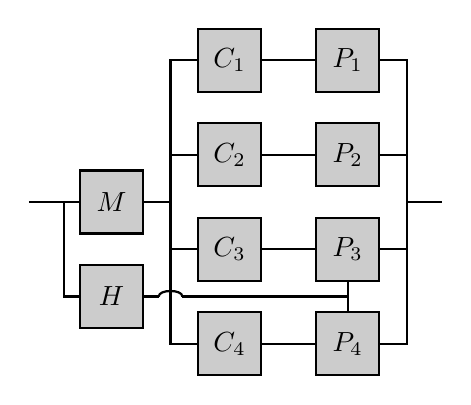
\begin{tikzpicture}
[typeM/.style={rectangle,draw,fill=black!20,thick,inner sep=0pt,minimum size=8mm}, %font=\footnotesize},
 typeC/.style={rectangle,draw,fill=black!20,thick,inner sep=0pt,minimum size=8mm}, %font=\footnotesize},
 typeP/.style={rectangle,draw,fill=black!20,thick,inner sep=0pt,minimum size=8mm}, %font=\footnotesize},
 typeH/.style={rectangle,draw,fill=black!20,thick,inner sep=0pt,minimum size=8mm}, %font=\footnotesize},
 type1/.style={rectangle,draw,fill=black!20,very thick,inner sep=0pt,minimum size=8mm},
 type2/.style={rectangle,draw,fill=black!20,very thick,inner sep=0pt,minimum size=8mm},
 type3/.style={rectangle,draw,fill=black!20,very thick,inner sep=0pt,minimum size=8mm},
 cross/.style={cross out,draw=red,very thick,minimum width=9mm, minimum height=7mm},
 hv path/.style={thick, to path={-| (\tikztotarget)}},
 vh path/.style={thick, to path={|- (\tikztotarget)}}]
\begin{scope}[xscale=1.5, yscale=1.2]
\node[typeM] (M)    at ( 0  , 0  ) {$M$};
\node[typeC] (C1)   at ( 1  , 1.5) {$C_1$};
\node[typeC] (C2)   at ( 1  , 0.5) {$C_2$};
%\node[cross]        at ( 1  , 0.5) {};
\node[typeC] (C3)   at ( 1  ,-0.5) {$C_3$};
%\node[cross]        at ( 1  ,-0.5) {};
\node[typeC] (C4)   at ( 1  ,-1.5) {$C_4$};
\node[typeP] (P1)   at ( 2  , 1.5) {$P_1$};
\node[typeP] (P2)   at ( 2  , 0.5) {$P_2$};
%\node[cross]        at ( 2  , 0.5) {};
\node[typeP] (P3)   at ( 2  ,-0.5) {$P_3$};
%\node[cross]        at ( 2  ,-0.5) {};
\node[typeP] (P4)   at ( 2  ,-1.5) {$P_4$};
\node[typeH] (H)    at ( 0  ,-1  ) {$H$};
\coordinate (start)  at (-0.7, 0);
\coordinate (startC) at ( 0.5, 0);
\coordinate (startH) at (-0.4, 0);
\coordinate (Hhop1)  at ( 0.4,-1);
\coordinate (Hhop2)  at ( 0.6,-1);
\coordinate (endP)   at ( 2.5, 0);
\coordinate (end)    at ( 2.8, 0);
\path (start)     edge[hv path] (M.west)
      (M.east)    edge[hv path] (startC)
      (startC)    edge[vh path] (C1.west)
                  edge[vh path] (C2.west)
                  edge[vh path] (C3.west)
                  edge[vh path] (C4.west)
      (C1.east)   edge[hv path] (P1.west)
      (C2.east)   edge[hv path] (P2.west)
      (C3.east)   edge[hv path] (P3.west)
      (C4.east)   edge[hv path] (P4.west)
      (endP)      edge[vh path] (P1.east)
                  edge[vh path] (P2.east)
                  edge[vh path] (P3.east)
                  edge[vh path] (P4.east)
                  edge[hv path] (end)
      (startH)    edge[vh path] (H.west)
      (H.east)    edge[hv path] (Hhop1)
      (Hhop1)     edge[thick,out=90,in=90] (Hhop2)
      (Hhop2)     edge[hv path] (P3.south)
                  edge[hv path] (P4.north);
\end{scope}
\end{tikzpicture}
\caption{Reliability block diagram for a simplified automotive brake system
with four component types $M$, $H$, $C$ and $P$.
Note that this system layout cannot be expressed as a nesting of series and parallel layouts.
The corresponding survival signature $\Phi(l_M,l_H,l_C,l_P)$ is given in Table~\ref{tab:brakesys-survsign}.}
\label{fig:brakesys-layout}
\end{figure}

In a system with $N$ components, the state of the components can be expressed by the state vector
$\vec{x} = (x_1,x_2,\ldots,x_N) \in \{0,1\}^N$,
with $x_i=1$ if the $i$th component functions and $x_i=0$ if not.
The structure function $\phi : \{0,1\}^N \rightarrow \{0,1\}$, defined for all possible $\vec{x}$,
takes the value 1 if the system functions and 0 if the system does not function for state vector $\vec{x}$ \citep{BP75}.
Most real-life systems are coherent,
which means that $\phi(\vec{x})$ is non-decreasing in any of the components of $\vec{x}$,
so system functioning cannot be improved by worse performance of one or more of its components.
Furthermore, one can usually assume that $\phi(0, \ldots, 0) = 0$ and $\phi(1, \ldots, 1) = 1$.

The survival signature \citep{2012:survsign} is a summary of the structure function
for systems with $K$ groups of exchangeable components.
Denoted by $\Phi(l_1,\ldots,l_K)$, with $l_k=0,1,\ldots,N_k$ for $k=1,\ldots,K$,
it is defined as the probability for the event that the system functions
given that precisely $l_k$ of its $N_k$ components of type $k$ function, for each $k\in \{1,\ldots,K\}$.
Essentially, this creates a $K$-dimensional partition for the event $\Tsys > t$,
such that $\Rsys(t) = P(\Tsys > t)$ can be calculated using the law of total probability,
\begin{align}
P(\Tsys > t) &= \sum_{l_1=0}^{N_1} \cdots \sum_{l_K=0}^{N_K} P(\Tsys > t \mid C^1_t = l_1,\ldots, C^K_t = l_K)
                                                                                  P\Big( \bigcap_{k=1}^K \{ C^k_t = l_k\} \Big) \nonumber\\
             &= \sum_{l_1=0}^{N_1} \cdots \sum_{l_K=0}^{N_K} \Phi(l_1,\ldots,l_K) P\Big( \bigcap_{k=1}^K \{ C^k_t = l_k\} \Big) \nonumber\\
             &= \sum_{l_1=0}^{N_1} \cdots \sum_{l_K=0}^{N_K} \Phi(l_1,\ldots,l_K) \prod_{k=1}^K P(C^k_t = l_k)\,,
\label{eq:sysrel-survsign}
\end{align}
where $P(C^k_t = l_k)$ is the (predictive) probability that exactly $l_k$ components of type $k$ function at time $t$,
and the last equality holds as we assume that components of different types are independent.
Note that for coherent systems, the survival signature $\Phi(l_1,\ldots,l_K)$ is non-decreasing in each $l_k$.

Continuing our example,
the survival signature for the system in Figure~\ref{fig:brakesys-layout} is given in Table~\ref{tab:brakesys-survsign},
omitting the entries for which $\Phi(l_M, l_H, l_C, l_P) = 0$ or $\Phi(l_M, l_H, l_C, l_P) = 1$,
since the full table would contain $\prod_{k=1}^K (N_k + 1) = 2 \times 2 \times 5 \times 5 = 100$ rows.

\begin{table}
\centering
\begin{tabular}{cccclcccccl}
  \toprule
M & H & C & P & $\Phi$ & \quad & M & H & C & P & $\Phi$\\ 
  \midrule
1 & 0 & 1 & 1 & 0.25 & & 1 & 0 & 2 & 1 & 0.50 \\ 
1 & 0 & 1 & 2 & 0.50 & & 1 & 0 & 2 & 2 & 0.83 \\ 
1 & 0 & 1 & 3 & 0.75 & & 1 & 0 & 3 & 1 & 0.75 \\ 
0 & 1 & 0 & 1 & 0.50 & & 1 & 1 & 0 & 1 & 0.50 \\ 
0 & 1 & 0 & 2 & 0.83 & & 1 & 1 & 0 & 2 & 0.83 \\ 
0 & 1 & 1 & 1 & 0.62 & & 1 & 1 & 1 & 1 & 0.62 \\ 
0 & 1 & 1 & 2 & 0.92 & & 1 & 1 & 1 & 2 & 0.92 \\ 
0 & 1 & 2 & 1 & 0.75 & & 1 & 1 & 2 & 1 & 0.75 \\ 
0 & 1 & 2 & 2 & 0.97 & & 1 & 1 & 2 & 2 & 0.97 \\ 
0 & 1 & 3 & 1 & 0.88 & & 1 & 1 & 3 & 1 & 0.88 \\ 
   \bottomrule
\end{tabular}
\caption{Survival signature $\Phi(l_M, l_H, l_C, l_P)$
for the simplified automotive brake system depicted in Figure~\ref{fig:brakesys-layout},
omitting the rows for which $\Phi(l_M, l_H, l_C, l_P) = 0$ or $\Phi(l_M, l_H, l_C, l_P) = 1$.}
\label{tab:brakesys-survsign}
\end{table}


\section{Adaptive system residual life distribution based on Weibull component models}
\label{sec:adaptive-sysrel-weibull}

In this section, we describe how the system reliability function $\Rsysnow(t)$ at current time $\tnow$ 
can be calculated for a specific choice of component model.
Section~\ref{sec:policy} will then show how an adaptive maintenance policy
can be derived for a monitored system based on such a current system residual life distribution. 

We consider the well-known Weibull model for component lifetimes,
which is used in a wide variety of reliability studies ***more motivation Weibull***. 
To keep things simple, we assume that the shape parameter of the Weibull distribution is known,
and that only the scale parameter needs to be estimated.
By using a Bayesian approach, described in Section~\ref{sec:weibull},
our component model allows to include both expert assessments and test data (if available),
and furthermore can account for component lifetime information from the current run of the system up to $\tnow$.
%***component model: weibull with fixed shape,
%inverse gamma prior on scale parameter,
%fix priors via expected lifetime and prior strength,
%test data inclusion
%with noninformatiove right-censoring
%
Section~\ref{sec:postpred} then derives the posterior predictive distribution
for the Weibull component model as needed for the current system reliability calculation.
Section~\ref{sec:sysreltnow} then adapts the method from Section~\ref{sec:sysrel} for the adaptive setting,
resulting in a formula for $\Rsysnow(t)$.
%***output is $\Rsysnow(t)$, the current (at time $\tnow$) system reliability function
%(residual life distribution, RLD)
%taking into account the current system state,
%including the current ages of system components, 
%and the lifetime histories of all component types,
%including test data (if available) and expert assessments.

The model description in this Section follows closely \cite{2016:walter-coolen},
who presented the same residual life distribution model.
However, \cite{2016:walter-coolen} do not consider any maintenance policies,
and focus instead on a generalization of the RLD model using sets of priors for the component models.
These sets of priors can be seen as parametric P-boxes,
a certain kind of imprecise probability model \citep[see, e.g.,][]{itip}.
Such models allow for vague and partial prior specifications,
and provide sensitivity to prior-data conflict \cite[\S 2.2.3.3]{diss}.


\subsection{Bayesian update of Weibull component models}
\label{sec:weibull}

Here we describe the Weibull model for the component lifetimes,
together with the Bayesian update procedure which allows to include
expert knowledge, component tests, and information from the currently monitored components in the system.

For each type $k$ component, we assume that the lifetime $T_{k,i}$ ($i=1,\ldots,N_k$, $k = 1, \ldots, K$)
is Weibull distributed with fixed shape parameter $\beta_k > 0$,
in short $T_{k,i} \mid \lambda_k \sim \wei(\beta_k,\lambda_k)$,
with density and cdf
\begin{align}
\label{eq:weibulldens}
f(t_{k,i} \mid \lambda_k) &= \frac{\beta_k}{\lambda_k} (t_{k,i})^{\beta_k-1} e^{-\frac{(t_{k,i})^{\beta_k}}{\lambda_k}}\,, \\
\label{eq:weibullcdf}
F(t_{k,i} \mid \lambda_k) &= 1 - e^{-\frac{(t_{k,i})^{\beta_k}}{\lambda_k}} = P(T_{k,i} \leq t_{k,i} \mid \lambda_k)\,,
\end{align}
where $\lambda_k > 0$ and $t > 0$.

The shape parameter $\beta_k$ determines whether the hazard rate is increasing ($\beta_k > 1$)
or decreasing ($\beta_k < 1$) over time.
For $\beta_k=1$, one obtains the Exponential distribution with constant hazard rate as a special case.
To keep things simple, we assume $\beta_k$ to be known.
(We plan to extend the model to learn also $\beta_k$ in a later step,
using, e.g., the discretized approach by \cite{1969:soland}.)
The scale parameter $\lambda_k$ can be interpreted through the relation
\begin{align}
\E[T_{k,i} \mid \lambda_k] &= \lambda_k^{1/\beta_k}\, \Gamma(1 + 1/\beta_k)\,.
\label{eq:lambdainterpret}
\end{align}
We will use this equation to convert expected lifetimes to $\lambda_k$ and vice versa.

With a Bayesian approach, one can express expert knowledge about the reliability of the components
by assigning a so-called prior distribution,
a distribution over the unknown parameter $\lambda_k$.
This prior distribution $f(\lambda_k)$ is then updated 
to the so-called posterior distribution $f(\lambda_k \mid \vec{t})$,
the distribution over $\lambda_k$ given the data $\vec{t}$,
via Bayes' rule
\begin{align*}
f(\lambda_k \mid \vec{t}) &\propto f(\vec{t}\mid\lambda_k) f(\lambda_k)\,.
\end{align*}
The posterior $f(\lambda_k \mid \vec{t})$ subsumes the information
from both expert knowledge and data,
and forms the basis for all inferences, like, e.g., predictions.

For the prior over $\lambda_k$,
a convenient choice is to use the inverse Gamma distribution,
which is commonly parametrized in terms of the parameters $a_k > 0$ and $b_k > 0$,
\begin{align}
f(\lambda_k\mid a_k,b_k) &= \frac{(b_k)^{a_k}}{\Gamma(a_k)} \lambda_k^{-a_k -1} e^{-\frac{b_k}{\lambda_k}}\,,
\label{eq:ig-def}
\end{align}
in short, $\lambda_k \mid a_k, b_k \sim \ig(a_k,b_k)$.
Here, we have added the prior parameters $a_k$ and $b_k$ in notation
to indicate that the prior over $\lambda$ depends on their values.

The inverse Gamma is convenient because it is a conjugate prior,
i.e., the posterior obtained by Bayes' rule is again inverse Gamma and thus easily tractable;
the prior parameters only need to be updated to obtain the posterior parameters,
so no numerical integation or simulation techniques are necessary.
Furthermore, this conjugacy holds also when right-censored observations are used for updating,
as indicated below.

In place of the usual parametrization in terms of $a_k$ and $b_k$,
we use the parameters $\nk > 1$ and $\yk > 0$
%(the upper index ${}\uz$ is used to indicate that these are prior parameters)
because they are more simple to interpret.
They are defined as
\begin{align}
\nk &= a_k - 1 & &\text{ and}
&
\yk &= b_k / \nk,
\label{eq:abtony}
\end{align}
where $\yk$ can be interpreted as the prior guess for the scale parameter $\lambda_k$,
as $\E[\lambda_k\mid\nk,\yk] = \yk$.
Using \eqref{eq:lambdainterpret},
we can thus translate an expert's statement of expected component lifetime into a corresponding value for $\yk$.
$\nk$ can be seen as a prior strength or pseudocount,
this will become clear in the discussion of the update step below.

The parametrization in terms of $\nk$ and $\yk$ also clarifies the nature of the combination
of prior information and data through Bayes' rule.
In the conjugate setting,
applying Bayes' rule simply means that the prior parameters $\nk$ and $\yk$
are updated to posterior parameters, which we denote by $\nkp$ and $\ykp$, respectively.
Assume we observe $N_k = e_k + c_k$ component lifetimes,
where $e_k$ is the number of actual failure events,
and $c_k$ is the number of right-censored observations.
We denote the failure times by $t_{k,1}, \ldots, t_{k,e_k}$,
and the censoring times by $t^+_{k,1}, \ldots, t^+_{k,c_k}$,
and collect them in an observation vector $\vec{t}_k = (t_{k,1}, \ldots, t_{k,e_k}, t^+_{k,1}, \ldots, t^+_{k,c_k})$.
Then, the updated, posterior parameters are
\begin{align}
\nkp &= \nk + e_k\,, 
&
\ykp &=  \frac{\nk \yk + \tautk}{\nk + e_k}\,,
\label{eq:ig-update}
\end{align}
where $\tautk = \sum_{i=1}^{e_k} (t_{k,i})^\beta + \sum_{i=1}^{c_k} (t^+_{k,i})^\beta$.
%The upper index ${}\un$ indicates that these are posterior parameters resulting from an update with $n_k$ observations,
%where we leave out the index $k$ for $n_k$ in the upper index to increase legibility.

From the simple update rule \eqref{eq:ig-update}, we see that
$\ykp$ is a weighted average of the prior parameter $\yk$ and the maximum likelihood (ML) estimator $\tautk/e_k$,
with weights proportional to $\nk$ and $e_k$, respectively.
$\nk$ can thus be interpreted as a prior strength or pseudocount,
indicating how much our prior guess should weigh against the $e_k$ observed failure events.
Furthermore, $\V[\lambda\mid\nk,\yk] = (\yk)^2 / (1 - 1/\nk)$;
for fixed $\yk$, a higher $\nk$ indicates thus 
that more probability mass is concentrated around $\yk$.

Using \eqref{eq:abtony} and \eqref{eq:ig-update}, the posterior distribution over $\lambda_k$ is
\begin{align}
\lambda_k \mid \nk, \yk, \vec{t}_k \sim \ig(\nk + e_k + 1, \nk \yk + \tautk)\,.
\label{eq:ig-update-alpha}
\end{align}
%where we have added the prior parameters $\nkz$ and $\ykz$ in notation
%to emphasize that the posterior is a synthesis of prior information and data.
As this posterior \eqref{eq:ig-update-alpha} can be defined in terms of
the updated, posterior parameters $\nkp$ and $\ykp$,
we may also write
\begin{align*}
f(\lambda_k \mid \nk, \yk, \vec{t}_k) &= f(\lambda_k \mid \nkp, \ykp)\,.
\end{align*}
The iterative nature of Bayesian inference means that we can take the updated,
posterior parameters as new prior parameters and update them again using new data.
Indeed, we will use this property to use the extra information about components
that accumulates during operation of the system:
At any time $\tnow > 0$,
all non-failed components correspond to a right censored observation $\tpnow$;
any failed components instead contribute a fully observed, non-censored lifetime,
and both types of observations can be used in the update step \eqref{eq:ig-update}.
%Before we write this out formally in Section~\ref{sec:postpred},
%we will first present how system reliability functions can be derived based on component models.

%To keep notation simple,
%we will below denote the parameters of the inverse Gamma distribution by $\nkz$ and $\ykz$,
%regardless of them expressing expert information alone,
%or stemming from the combination of expert information and test data.


\subsection{Component posterior predictive distributions at $\tnow$}
\label{sec:postpred}

To calculate the current system reliability function $\Rsysnow(t)$,
we need, for each $k=1,\ldots, K$, the probabilities $P(C^k_t = l_k)$
for the number of type $k$ components that function at times $t > \tnow$,
taking into account all information available at $\tnow$.
In the Bayesian framework, these probabilities are given
by a so-called posterior predictive distribution that can be derived from the posterior over $\lambda$.

Denote by $\nkz$ and $\ykz$ the parameters reflecting the knowledge base at system start-up time $t=0$.
These could have been obtained by updating prior parameters $\nk$ and $\yk$ (reflecting expert knowledge)
to $\nkp$ and $\ykp$ using test data,
or could be taken directly equal to $\nk$ and $\yk$ if no test data is available.
In both cases, the distribution $f(\lambda_l \mid \nkz, \ykz)$
thus accounts for all knowledge on component type $k$ that is available at system start-up.

Following our comments at the end of Section~\ref{sec:weibull},
the component models can be further updated
using information gained from the current run of the system until $\tnow$:
Any failure times of failed components,
and the right-censoring time $\tpnow$ for each non-failed component,
can be used to update $\nkz$ and $\ykz$ according to \eqref{eq:ig-update}.
We denote the resulting parameter values by $\nknow$ and $\yknow$.
%(It is of course possible to update $\nkz$ and $\ykz$ directly to $\nknow$ and $\yknow$ if no test data is available.)
%Furthermore, the fact that the components in the system that still function have reached the age $\tnow$
%must be used when calculating the posterior predictive distribution.

In analogue to the notation from Section~\ref{sec:weibull},
let $N_k = \eknow + \cknow$ be the number of type $k$ components in the monitored system,
where $\eknow$ is the number of components that have failed by $\tnow$,
and $\cknow$ is the number of components that have not failed by $\tnow$.
We can thus collect these observations, as of $\tnow$, in a vector
$\vectknow = (t_{k,1}, \ldots, t_{k,e_k}, \tpnow, \ldots, \tpnow)$,
containing $\cknow$ right-censored observations $\tpnow$.
%
The resulting posterior predictive distribution for any $t > \tnow$ is obtained as
\begin{align}
\lefteqn{%
P(C^k_t = l_k\mid\nkz,\ykz, \vectknow) }\hspace*{5.75ex} \nonumber\\  %
 &= { \cknow \choose l_k} \int \big[P(T^k >    t \mid T^k > \tnow, \lambda_k)\big]^{l_k} \times \nonumber\\ & \hspace*{3.5ex}
                               \big[P(T^k \leq t \mid T^k > \tnow, \lambda_k)\big]^{\cknow - l_k}
    f(\lambda_k\mid\nkz,\ykz,\vectknow) \dd \lambda_k\,,
\label{eq:postpredtnow}
\end{align}
where $T^k$ is the Weibull distributed lifetime of a component of type $k$.
Note that through the condition $T^k > \tnow$, we also take into account
that the components in the system have the age $\tnow$.
Now, by the Weibull assumption \eqref{eq:weibullcdf}, one has
\begin{align}
P(T^k \leq t \mid T^k > \tnow, \lambda_k)
 &= \frac{P(\tnow < T^k \leq t \mid\lambda_k)}{P(T^k > \tnow \mid \lambda_k)} \nonumber\\
 &= \frac{F(t\mid\lambda_k) - F(\tnow\mid\lambda_k)}{1-F(\tnow\mid\lambda_k)} 
% = \frac{e^{-\frac{(\tnow)^{\beta_k}}{\lambda_k}} - e^{-\frac{t^{\beta_k}}{\lambda_k}}}{e^{-\frac{(\tnow)^{\beta_k}}{\lambda_k}}}
  = 1 - e^{-\frac{t^{\beta_k} - (\tnow)^{\beta_k}}{\lambda_k}}\,.
\label{eq:weibullcondprob}
\end{align}
Substituting \eqref{eq:weibullcondprob} and the posterior \eqref{eq:ig-update-alpha} using $\vectknow$,
written in terms of the updated parameters $\nknow$ and $\yknow$,
into \eqref{eq:postpredtnow}, we get
\begin{align}
\lefteqn{P(C^k_t = l_k\mid\nkz,\ykz, \vectknow)}\hspace*{5.75ex} \nonumber\\
 &= { \cknow \choose l_k} \int \Big[    e^{-\frac{t^{\beta_k} - (\tnow)^{\beta_k}}{\lambda_k}}\Big]^{l_k}
                               \Big[1 - e^{-\frac{t^{\beta_k} - (\tnow)^{\beta_k}}{\lambda_k}}\Big]^{\cknow - l_k}
    \times \nonumber\\ & \hspace*{14.5ex}
    \frac{\big(\nknow\yknow\big)^{\nknow + 1}}{\Gamma(\nknow + 1)}
    \lambda_k^{-(\nknow + 1) - 1} e^{-\frac{\nknow\yknow}{\lambda_k}} \dd \lambda_k \nonumber\\
 &= { \cknow \choose l_k} \sum_{j=0}^{\cknow - l_k} (-1)^j { \cknow - l_k \choose j}
    \frac{\big(\nknow\yknow\big)^{\nknow + 1}}{\Gamma(\nknow + 1)} 
    \times \nonumber\\ & \hspace*{1ex}
    \int \lambda_k^{-(\nknow + 1) - 1}
    \exp\Big\{-\frac{(l_k + j) (t^{\beta_k} - (\tnow)^{\beta_k}) + \nknow\yknow}{\lambda_k}\Big\} \dd \lambda_k\,.
\end{align}
The terms remaining under the integral form the core of an inverse gamma distribution \eqref{eq:ig-def}
with parameters $\nknow + 1$ and $\nknow\yknow + (l_k + j) (t^{\beta_k} - (\tnow)^{\beta_k}))$,
allowing to solve the integral using the corresponding normalization constant.
We thus have, for $l_k \in \{0,1,\ldots,\cknow\}$,
\begin{align}
\label{eq:postpred-priorparams}
\lefteqn{P(C^k_t = l_k\mid\nkz,\ykz, \vectknow)}\hspace*{5ex} \nonumber\\
 &= { \cknow \choose l_k} \sum_{j=0}^{\cknow - l_k} (-1)^j { \cknow - l_k \choose j} \times \nonumber\\ & \hspace*{10ex}
    \left(\frac{\nknow\yknow}{\nknow\yknow + (l_k + j) \big(t^{\beta_k} - (\tnow)^{\beta_k}\big)}\right)^{\nknow + 1} \,, \\
 & \quad\text{where } \nknow\yknow = \nkz\ykz + \sum_{i=1}^{\eknow} (t_{k,i})^{\beta_k} + \cknow (\tnow)^{\beta_k} \nonumber\\
 & \quad\text{and }  \nknow = \nkz + \eknow \,. \nonumber
% &= { \cknow \choose l_k} \sum_{j=0}^{\cknow - l_k} (-1)^j { \cknow - l_k \choose j} \times \nonumber\\ & \hspace*{1ex}
%    \left(\frac{\nkz\ykz + \sum_{i=1}^{\eknow} (t_{k,i})^{\beta_k} + \cknow (\tnow)^{\beta_k} }%
%               {\nkz\ykz + \sum_{i=1}^{\eknow} (t_{k,i})^{\beta_k} + \cknow (\tnow)^{\beta_k} +%
%                (l_k + j) \big(t^{\beta_k} - (\tnow)^{\beta_k}\big) }\right)^{\nkz + \eknow + 1}.
% &= \sum_{j=0}^{\cknow - l_k} (-1)^j \frac{\cknow !}{l_k! j! (\cknow - l_k - j)!}   
%    \left(\frac{\nknow\yknow}{\nknow\yknow + (l_k + j) \big(t^{\beta_k} - (\tnow)^{\beta_k}\big)}\right)^{\nknow + 1} \nonumber\\
% &= \sum_{j=0}^{\cknow - l_k} (-1)^j \frac{\cknow !}{l_k! j! (\cknow - l_k - j)!} \times \nonumber\\ & \hspace*{10ex}  
%    \left(\frac{\nkz\ykz + \sum_{i=1}^{\eknow} (t_{k,i})^{\beta_k} + \cknow       (\tnow)^{\beta_k} }%
%               {\nkz\ykz + \sum_{i=1}^{\eknow} (t_{k,i})^{\beta_k} + (\cknow - l_k - j) (\tnow)^{\beta_k} + (l_k + j) t^{\beta_k} }\right)^{%
%    \nkz + \eknow + 1}.
\end{align}
%where $\nknow\yknow = \nkz\ykz + \sum_{i=1}^{\eknow} (t_{k,i})^{\beta_k} + \cknow (\tnow)^{\beta_k}$
%and $\nknow = \nkz + \eknow + 1$.
%These posterior predictive probabilities can also be expressed as a cumulative probability mass function (cmf)
%\begin{align}
%F(l_k \mid \nkz,\ykz,\vectknow) = P(C^k_t \leq l_k \mid \nkz,\ykz,\vectknow) 
% = \sum_{j=0}^{l_k} P(C^k_t = j \mid \nkz,\ykz,\vectknow)\,.
%\end{align}


\subsection{System reliability function at $\tnow$}
\label{sec:sysreltnow}

Now that we can calulate the component posterior predictive distributions at $\tnow$,
we can use the method from Section~\ref{sec:sysrel}
to determine the system reliability distribution $\Rsysnow(t)$,
giving us the probability that the system functions at times $t > \tnow$,
taking into account all information available at $\tnow$:
\begin{align}
\Rsysnow(t) &= \sum_{l_1=0}^{c_1^{(\tnow)}} \cdots \sum_{l_K=0}^{c_K^{(\tnow)}} \Phinow(l_1,\ldots,l_K)
               \prod_{k=1}^K P(C^k_t = l_k\mid\nkz,\ykz, \vectknow)\,.
\label{eq:sysrel-tnow}
\end{align}
Note that if one or several components have failed by $\tnow$,
the system layout changes, and with it the survival signature $\Phi(l_1,\ldots,l_K)$,
so we denote the updated survival signature by $\Phinow(l_1,\ldots,l_K)$.

For each prediction time $t$,
\eqref{eq:sysrel-tnow} is a sum over over $\prod_{k=1}^K (\cknow + 1)$ terms;
however, some of these terms correspond to $\Phinow(l_1,\ldots,l_K) = 0$,
which can thus be disregarded.
For each of the remaining terms,
we must calculate the product $\prod_{k=1}^K P(C^k_t = l_k\mid\nkz,\ykz, \vectknow)$.
For all products, the constituting factors can be taken from the same table
enumerating $P(C^k_t = l_k\mid\nkz,\ykz, \vectknow)$ for all $l_k \in \{0, 1, \cknow\}$, $k=1\ldots,K$,
so \eqref{eq:postpred-priorparams} needs to be invoked 
only $\sum_{k=1}^K (\cknow + 1)$ times.

We will evaluate \eqref{eq:sysrel-tnow} on a dense grid of prediction times $t > \tnow$,
thus discretely approximating the RLD.
As the evaluation of \eqref{eq:sysrel-tnow} for each $t$ does not involve any complex numeric calculations or Monte Carlo sampling,
the grid of prediction values can be very fine.

Next, we will describe how an adaptive maintenance policy based on %\eqref{eq:sysrel-tnow}
a current residual life distribution,
first in general, then for our implementation,
where a fine discrete approximation of the RLD is obtained.


\section{Dynamic and adaptive maintenance policy based on the current system residual life distribution}
\label{sec:policy}

We can now derive the adaptive and dynamic maintenance policy
that resembles a CBM policy.
However, instead of determining a threshold for a degradation signal like in usual CBM approaches,
we determine, for each present time $\tnow$,
the adaptive and dynamic timespan $\tausnow$ which gives the time from $\tnow$ until the optimal moment of maintenance.
Close to system startup, $\tausnow$ will be large;
but as components in the system age and some indeed fail over time,
$\tausnow$ will typically decrease.
Let $\tprep$ be the timespan needed to prepare maintenance work.
As soon as $\tausnow$ decreases below $\tprep$,
a preventive maintenance action is initiated.
This operational procedure is described in more detail in Section~\ref{sec:operationalprocedure}.
%and executed at time $\tnow + \tausnow$.

***comments about `nervousness' of $\tausnow$ here or in \ref{sec:operationalprocedure}?
common cause failures currently not in the model, but will seriously influence residual life distribution,
see comments in Outlook (Section~\ref{sec:outlook})

The optimal time to maintenance $\tausnow$ is determined based on $\Rsysnow(t)$
by minimizing $\gnow(\tau)$, the expected unit cost rate for the current operational cycle.
(An operational cycle begins with system start-up,
and ends when either a failure of the system occors, or a preventive maintenance is carried out.)
This criterion, as described in Section~\ref{sec:costrate} below in detail,
only assumes that $\Rsysnow(t)$ is given,
and thus is not tied to our choice of component model.
One could also consider other optimality criteria to determine $\tausnow$.
When safety is paramount one could, e.g., determine $\tausnow$ such that
the probability of system failure is at most at some very low pre-determined level.

Section~\ref{sec:optim} then focuses on our choice of component model and the resulting form for $\Rsysnow(t)$,
and shows how $\tausnow$ is determined in this situation.
Numerical examples for different failure histories are given in Section~\ref{sec:examples}.


\subsection{Operational Procedure}
\label{sec:operationalprocedure}

***illustrative figure?

Each operational cycle starts with system startup.
At this point in time, the system is in an (as good as) new state,
i.e., all components in the system are (as good as) new and have not aged.
A cycle ends when the system is either maintained preventively, %at time $\tnow + \tausnow$ (on an absolute time scale),
or the system fails, which triggers a corrective maintenance action.

During a cycle,
$\tausnow$ is recalculated at a frequency small enough to be negligible on the system lifetime scale.
This is feasible because we use a fast discrete approximation of the unit cost rate function $\gnow(\tau)$,
and determine $\tausnow$ with a simple grid search.
Updating $\tausnow$ frequently is useful because,
even in absence of failures of system components,
all components age, and also non-failure adds information to the component models.
Both aspects influence $\Rsysnow(t)$ and thus $\tausnow$.
%An alternative would be to update $\tausnow$ only when a component fails,
%but as a (near) real-time update of $\taausnow$ is possible and useful,
%as non-failed components still can be used to update component models ($\nknow$ and $\yknow$) via right-censored observation $\tpnow$.

The calculation of $\tausnow$ for a fixed $\tnow$ resembles the calculation
of the maintenance interval in an age based policy;
however, because $\tausnow$ is derived from the current $\Rsysnow(t)$,
our policy is adaptive and dynamic like a CBM policy. 
Like in an age-based policy, the derived $\gnow(\tau)$ can also be monotonely decreasing.
In this case, it is, at the moment $\tnow$, optimal to correctively maintain the system.
This means that our approach is not only capable of finding the optimal moment for preventive maintenance,
but also capable of indicating when corrective maintenance is the better option.
%i.e., capable of choosing the maintenance policy.

A preventive maintenance action is triggered as soon as $\tausnow$ falls below $\tprep$,
the time needed to prepare maintenance work.
The system continues to run until maintenance work begins,
and the cycle ends when maintenance work is completed.
When the system fails, instead a corrective maintenance action is triggered,
and the system is down also during the wait until maintenance work begins.
This additional downtime must be reflected in the cost parameter $c_u$ (see Section~\ref{sec:costrate} below).
Again, the cycle ends when maintenance work is completed.

At the end of each cycle,
the component information gained during the completed cycle is added to the component knowledge base
by updating the parameters $\nk$ and $\yk$ accordingly,
%using failure and censoring times as of the end of the cycle.
such that $\nkz$ and $\ykz$ for the following cycle account for the (censored) lifetimes observed during the previous cycle.
%We assume that both planned and unplanned maintenance action takes negligible time,
We assume that both a planned and unplanned maintenance action results in an (as good as) new system state by replacing all components,
such that the system begins a new cycle always under the same conditions.
Replacement schemes that do not replace all components would require to account for the different ages of components in the system
at the start of a new cycle.
While this is in principle possible in our approach,
exploring such selective replacement schemes is out of scope for this paper,
since optimizing over replacement schemes is, in our view, a higly interesting topic on its own,
and we will comment on this in the Outlook (Section~\ref{sec:outlook}).

As we use a one-cycle criterion, the time both planned and unplanned maintenance actions require
does not matter directly for the determination of $\tausnow$.
Downtimes are instead accounted for indirectly via the costs parameters in the trade-off leading to $\tausnow$,
as described next.

%To find the optimal moment for maintenance based on the current system reliability function $\Rsysnow(t)$,
%we minimize the expected average cost per time unit,
%called the unit cost rate, $g(\tau)$,
%leading to the cost-optimal moment of maintenance $\tau_*$.
%(could be discounted as well, out of scope here.)


\subsection{Expected unit cycle cost rate}
\label{sec:costrate}

To determine the optimal time to maintenance $\tausnow$,
we use the expected one-cycle cost rate 
\citep{1984:ansell-bendell-humble,1996:mazzuchi-soyer,2006:coolen-schrijner-coolen}
as the unit cost rate.
Although a different, renewal theory based way to calculate the unit cost rate is often used
in CBM literature \citep[e.g.,][]{2013:si-et-al,2011:kim-et-al},
%As we discussed in the Introduction,
we use the one-cycle cost rate as it is the most appropriate for our situation,
where $\tausnow$ changes with every cycle, and indeed changes with $\tnow$ within each cycle.
%since it considers only the costs with respect to the current cycle.

Let $c_p$ be the cost of planned (preventive) maintenance, and $c_u$ the cost of unplanned (breakdown) maintenance, where $c_p < c_u$.
Usually, set-up costs, work costs and downtime costs are much higher for unplanned / breakdown maintenance,
such that often, $c_p \ll c_u$.
CBM is known to be most effective when the difference between $c_p$ and $c_u$ is large
(***cite de Jonge and Teunter working paper on relative benefit).
%
As discussed above,
we assume that both $c_p$ and $c_u$ include the cost of replacing all components in the system.
That means that every time a new cycle starts, the system is in the same state with all components (as-good-as) new.

Let $\Tsysnow$ be the random variable corresponding to $\Rsysnow(t)$,
giving the (random) system failure time for times $t > \tnow$,
conditioned on all information available at $\tnow$,
and $\fsysnow(t)$ be the corresponding density.
Conditional on the realization $\tsysnow$ of $\Tsysnow$, the unit cost rate is 
\begin{align}
g(\tau \mid \Tsysnow = \tsysnow) &=
\begin{cases}
c_p / \tau     & \text{if } \tsysnow \ge \tnow + \tau \\
c_u / \tsysnow & \text{if } \tsysnow  <  \tnow + \tau \,.
\end{cases}
\label{eq:gtau}
\end{align}
Note that here, $\tau$ is a timespan starting from $\tnow$,
and so is a time on a prospective time scale, where $0$ corresponds to $\tnow$.
In contrast, $\tnow$ and $\tsysnow$ are times on an absolute time scale,
where $0$ corresponds to the time of system start-up.
Taking the expectation over $\Tsysnow$ in \eqref{eq:gtau} leads to the expected unit cost rate being
\begin{align}
\gnow(\tau) &= \E[g(\tau \mid \Tsysnow)] = \frac{c_p}{\tau} \Rsysnow(\tau) + c_u \int_0^\tau \frac{1}{t} \fsysnow(\tnow + t) \dd t\,,
\label{eq:gtnowtau}
\end{align}
and $\tausnow = \arg\min \gnow(\tau)$.
$\tausnow$, the optimal moment of maintenance as of $\tnow$,
incorporates thus all that is known at current time $\tnow$.
%The lower index $\tnow$ of $\tausnow$ emphasizes that
%depends on $\tnow$, and also on the history of the system.
Figure~\ref{fig:ghistfig2} illustrates this procedure for a number of current times $\tnow$.

Note that for the integral in \eqref{eq:gtnowtau} to exist, $\E[1/\Tsysnow \mid \Tsysnow > \tnow]$ must exist,
which is a condition for $\fsysnow(\tnow + t)$ for values of $t$ close to $0$ \citep{2006:coolen-schrijner-coolen}.
This restriction probably plays a role in the CBM literature's reluctance to adopt the one-cycle criterion.
For our approach, however, this condition is not relevant,
as we use a discrete approximation of $\Rsysnow(t)$ and $\fsysnow(t)$, respectively
(see Section~\ref{sec:optim} below).

Minimizing $\gnow(\tau)$ leads to $\tausnow$,
the optimal moment of maintenance on a prospective time scale.
The prospective unit cost rate $\cstarnow = \gnow(\tausnow)$ corresponding to $\tausnow$
thus is the lowest unit cost rate attainable for the span of the remaining lifetime of the system,
i.e., for what happens beyond current time $\tnow$.
Also of interest is the total cost rate at $\tnow$, denoted by $\ctotalnow$.
This gives the expected unit cost rate calculated over the full time since system start-up,
under the assumption that maintenance is scheduled for $\tstarnow = \tnow + \tausnow$.
$\ctotalnow$ generally decreases with $\tnow$ since for larger $\tnow$, maintenance costs are spread over a longer time.
However, when many (or few but critical) components fail, $\ctotalnow$ may increase,
since then, system failure becomes much more likely, leading to a higher $\cstarnow$.
For a numerical example, these relations are depicted in Figure~\ref{fig:tauhistfig2}.

We will describe next how we numerically evaluate \eqref{eq:gtnowtau} and find $\tausnow$
for our choice of component model.
%($\beta_k > 1$ $\forall k = 1,\ldots,K$ sufficient **???**)
%***here, $\Rsysnow(\cdot)$ shifted such that $\tnow = 0$.


\subsection{Numerical optimization of the expected unit cycle cost rate}
\label{sec:optim}

Since $\Rsysnow(t)$ is not tractable analytically,
we calculate $\Rsysnow(t)$ for values of $t$ on a dense grid spanning from $\tnow$ to some horizon time $\tnow + t_h$.
(The choice of $h_t$ is discussed in more detail below.)
We calculate $\gnow(\tau)$ on the same grid,
and determine $\tausnow$ by minimizing over this grid.
Here, we approximate the integral in \eqref{eq:gtnowtau} numerically by a sum,
where $\fsysnow(t)$ is calculated via differences of $\Rsysnow(t)$ values on the grid.
%$\gnow(\tau)$ is likewise evaluated on a dense grid,
%and $\tausnow = \arg\min \gnow(\tau)$ is determined as the minimum over the grid.

The horizon span $t_h$ can be determined by practical considerations,
but generally should reach far enough into the tail of $\Rsysnow(t)$
such that $\gnow(\tau)$ is not cut off before it reaches its minimum. %one can be sure to find $\tausnow$.
Note that from \eqref{eq:gtnowtau} it is clear that one needs only ****


***calculations in \textsf{R} can be vectorized and are thus fast.

***if min $\gnow(\tau)$ at $\tnow + t_h$, corrective maintenance is optimal: policy switch!
%***if $\tau_*^{(\tnow)}$ larger than certain horizon, than conclude corrective policy

%At time $\tnow$, the corresponding $\tausnow$ gives the optimal moment of maintenance in terms of time to elapse after $\tnow$,
%so in the absolute time scale, the optimal moment of maintenance is at $\tnow + \tau_*^{\tnow}$.


\begin{figure}
\includegraphics[width=\textwidth]{ghistfig2}
\caption{System reliability and unit cost rate functions for $\tnow = 0,2,4,6,8$
for the system depicted in Figure~\ref{fig:brakesys-layout}
and prior component models as given in Table~\ref{tab:priorparams},
assuming the failure history $P_2 = 3$, $P_3 = 4$, $C_2 = 6$, $C_3 = 7$, $H = 8$,
and costs $c_u = 1$, $c_p = 0.2$.}
\label{fig:ghistfig2}
\end{figure}


\section{***numerical examples for complex system layout}
\label{sec:examples}

***use simplified brake system from ASCE-ASME paper,
different example histories (when do components fail?)

***In current graphs,
prior component model parameters are taken as in Table~\ref{tab:priorparams},
and $c_u = 1$, $c_p = 0.2$. *** plot prior predictive distributions?***

***example figures are with very weak prior info
(see Table~\ref{tab:priorparams}: $\nkz = 1$ or $2$),
things could look different for stronger expert information!

***also example where remaining component type is (close to) exponential,
such that corrective maintenance becomes optimal!

\begin{table}
\centering
\begin{tabular}{crrrrrrr}
  \toprule
$k$ & $\beta_k$ & $\E[T_i^k]$ & $\ykz$ & $\nkz$ \\
  \midrule
M & $2.5$ & $5$\rule{1.5ex}{0ex} & $75.4$ & $2$\rule{1ex}{0ex} \\
H & $1.2$ & $2$\rule{1.5ex}{0ex} & $ 2.5$ & $1$\rule{1ex}{0ex} \\
C & $2  $ & $8$\rule{1.5ex}{0ex} & $81.5$ & $1$\rule{1ex}{0ex} \\
P & $1.5$ & $3$\rule{1.5ex}{0ex} & $ 6.1$ & $1$\rule{1ex}{0ex} \\
  \bottomrule
\end{tabular}
\caption{Prior parameters for the four component types as used in subsequent numerical examples.
The corresponding expected failure behaviour is visualized in Figure~\ref{fig:comppriorfig1}.}
\label{tab:priorparams}
\end{table}

\begin{figure}
\centering
\includegraphics[width=0.8\textwidth]{comppriorfig1}
\caption{Prior predictive reliability functions corresponding to the values from Table~\ref{tab:priorparams},
%for the four component types of the system depicted in Figure~\ref{fig:brakesys-layout},
showing the expected failure behaviour according to this choice of parameters.}
\label{fig:comppriorfig1}
\end{figure}

\begin{figure}
\includegraphics[width=\textwidth]{tauhistfig2}
\caption{$\tausnow$, $\tstarnow = \tnow + \tausnow$, $\cstarnow = \gnow(\tausnow)$,
and the total unit cost rate $\ctotalnow$ as functions of $\tnow$
for the system depicted in Figure~\ref{fig:brakesys-layout},
assuming the failure history $P_2 = 3$, $P_3 = 4$, $C_2 = 6$, $C_3 = 7$, $H = 8$,
and $c_u = 1$, $c_p = 0.2$.
$\tausnow$ (top left panel) first decreases slightly, then remains more or less constant during failure-free periods,
dropping significantly at the failures of components $P_2$, $P_3$ and $H$ only.
If $\tprep = 0.5$, the drop of $\tausnow$ from $0.72$ to $0.38$ at $\tnow = 8$ would trigger a maintenance action
at (absolute) time $8.5$.
Since $\tausnow$ does not change dramatically most of the time, $t^*$,
the cost-optimal moment of maintenance on the absolute timescale (top right panel),
steadily increases, with small drops corresponding to drops in $\tausnow$,
indicating that as time progresses, accumulated information indicates that maintenance can be postponed.
Note that $\gnow(\tausnow)$ is the momentary cost rate relating to the expected residual lifetime (lower left panel),
differing from the overall cost rate $\ctotalnow$ (lower right panel).
%For the maintenance action triggered at $\tnow = 8$,
%the overall cost rate is $c_p / 8.5 = 0.024$ if the system does not fail until time $8.5$,
%and between $c_u / 8 = 0.125$ and $c_u / 8.5 = 0.118$ if the system fails.}
At time $8$, the overall expected cost rate for repair scheduled at time $8.38$ is $0.044$,
up from $0.036$ for repair scheduled at time $8.62$, as cost-optimal at time $7.9$.}
\label{fig:tauhistfig2}
\end{figure}

\begin{figure}
\includegraphics[width=\textwidth]{tauhistfig3}
\caption{Illustration of the gains due to the parameter update
assuming the failure history $P_2 = 3$, $P_3 = 4$, $C_2 = 6$, $C_3 = 7$, $H = 8$.
$\tausnow$ (top left panel) is consistently lower for the non-adaptive algorithm,
same with $t^*$ (top right panel).
The adaptive algorithm recongnizes the higher reliability of system components,
leading to lower current (lower left panel) and total (lower right panels) unit cost rates.}
\label{fig:tauhistfig3}
\end{figure}


\begin{figure}
\includegraphics[width=\textwidth]{tauhist2fig3}
\caption{***early failures: $C_2 = 1$, $C_2 = 3$, $P_2 = 0.5$, $P_3 = 1.5$}
\label{fig:tauhist2fig3}
\end{figure}

\begin{figure}
\includegraphics[width=\textwidth]{tauhist3fig3}
\caption{***very late failures: $C_2 = 10$, $C_3 = 12$, $H = 14$, $P_2 = 8$, $P_3 = 9$}
\label{fig:tauhist3fig3}
\end{figure}


***larger simulation study?


\section{Outlook}
\label{sec:outlook}

***$\tprep$ could vary over time, e.g., longer on weekends or outside office hours

*** study other replacement schemes, e.g., replacing only failed components:
when repaired/replaced components are present in system,
then one needs to use actual ages (and not time since system startup) in parameter update,
introduces new component type for $\Rsysnow(t)$ calculation but with same posterior parameters as unreplaced component type.
Repaired/replaced components require the creation of a separate type in the survival signature decomposition
and thus the calculation of separate posterior predictive probabilities
$P(C^k_t = l_k \mid \nkz,\ykz,\vectknow)$,
which use, however, the same hyperparameter learning (using actual component ages) as the `parent type'.

***common-cause failures will seriously reduce RLD in a way currently not covered by our model.
This needs to be implemented on the level of component models,
specifically $P\Big( \bigcap_{k=1}^K \{ C^k_t = l_k\} \Big)$ 
(not a product anymore if common-case failures can affect several component times at once).
Combine ideas from \cite{2015:coolen-coolen-maturi} and \cite{Troffaes2014a}.

*** move to sets of priors, set of residual life distributions like in \cite{2016:walter-coolen}.
Leads to set of $\gnow(\tau)$, finding (set of) $\tausnow$ is then non-trivial,
needs decision criteria from imprecise probability literature like E-admissibility, maximality, or maximin
\citep[see, e.g., \S 9***][]{itip}.

*** to use the model for inspection-based CBM (if no repair necessary, find optimal timing of next inspection),
we would need to add interval-censored data (failure has happened between last and current inspection)




\section*{Acknowledgements}

CAMPI

Frank Coolen for inspiring discussions

\section*{Bibliography}

\bibliographystyle{elsarticle-harv}

\bibliography{refs}

\end{document}
